\section{Movie script dataset}
\label{fire}

Following prior work on personalized dialogue systems, we explore the applicability of fictional dialogues from TV or movie scripts to approximate real-life conversations \cite{li2016persona, lin2011all}. Movie scripts are a practical source of transcribed conversations because they are freely available, dialogue-intensive, and each utterance has the speaker marker (unlike, for example, dialogues in novels). Exemplary conversations from popular movies are shown in Figure~\ref{fig:movie-script}. 

Specifically, we created two datasets consisting of characters' utterances: Movie Character Attributes dataset (MovieChAtt), labeled with speakers' demographic attributes (\textit{age}, \textit{gender}, \textit{profession}), and Film Relationship dataset (FiRe), labeled with characters' \textit{interpersonal relationships}.

\begin{figure}[h!]
\RawFloats
\centering
\begin{minipage}[t]{0.47\textwidth}
\centering
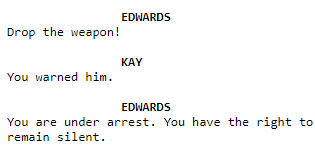
\includegraphics[width=1.0\textwidth]{data/pics/men in black.png}
\vspace*{-3mm}
\caption*{{\small \textbf{Excerpt from ``Men in Black'' (1997)}}}
\label{fig:2figsA}
\end{minipage}
\qquad
\begin{minipage}[t]{0.45\textwidth}
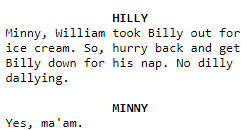
\includegraphics[width=0.9\textwidth]{data/pics/the help.png}
\vspace*{2mm}
\caption*{{\small \textbf{Excerpt from ``The Help'' (2011)}}}
\label{fig:2figsB}
\end{minipage}
\caption{Examples of conversations in the movie scripts.}
\label{fig:movie-script}
\end{figure}


\subsection{Related work}

In this section we give a brief overview of the existing conversational datasets of speaker's personal attributes and interpersonal relationships. We outline their shortcomings, which we addressed by collecting our own datasets.

\subsubsection{Datasets of demographic traits} 

Many conversational datasets labeled with personal attributes are not publicly available due to privacy protection of the speakers' data. The few accessible datasets include spoken dialogue transcriptions \cite{cieri2004fisher, love2017spoken} and artificially created conversations \cite{zhang2018personalizing, pers2}.

\citet{cieri2004fisher} gathered transcribed telephone dialogues on the given general topics; each speaker indicated their age, gender, dialect, education and occupation. \citet{love2017spoken} created a corpus of transcribed casual conversations of British English speakers, where all speakers specified their demographic (\textit{age}, \textit{nationality}, etc) and linguistic attributes (\textit{mother tongue}, \textit{dialect}). 

\citet{pers2} introduced an extension to the bAbI goal-oriented user-chatbot dialogue dataset \cite{bordes2016learning}, providing the users' ages, genders and food preferences. \citet{zhang2018personalizing} created a crowdsourced conversation dataset, Persona-Chat, where each speaker had to employ the given personality, described with a few sentences. A drawback of Persona-Chat is that it provides only textual descriptions of personas, as opposed to precise demographic facts. 
In general, the conversations created in a controlled way sound artificial, lacking of natural topic drifts and unnecessarily emphasizing the required content.  

\subsubsection{Datasets for relationship prediction} 

Two popular sources of conversational data for interpersonal relationship inference, are literary texts and movie scripts. Several studies provided the annotated relationships of the characters in novels as binary labels (positive or negative sentiment) \cite{chaturvedi2016modeling} or described as a bag-of-words \cite{iyyer2016feuding}. \citet{massey2015annotating} annotated the characters in literary texts with relationships on different granularity, additionally indicating the temporal change in relationship. 

Compared to literary texts, movie and series scripts provide dialogues in a structured format, simplifying speakers' identification. \citet{chen2020mpdd} collected conversations from Chinese TV series scripts and used three annotators to label them with 24 relationships and 7 emotions. The relationship labels were hierarchically split by field (\textit{family}, \textit{school}, \textit{company}, \textit{other}) and seniority (\textit{elder}, \textit{peer}, \textit{junior}). TV series scripts were also used by \citet{yu-etal-2020-dialogue}, where the script of Friends series was annotated by 2 judges with 36 predicates for relation extraction task, where 14 of the predicates indicated the relationship between people. \citet{jia2020ddrel} annotated relationships of the characters in the movie scripts with 13 relationship labels, belonging to four main categories (\textit{family}, \textit{intimacy}, \textit{official}, \textit{others}), resulting in the DDRel dataset. 

Unlike most prior works, we consider \emph{directed} relationships (e.g., \emph{parent} and \emph{child} as separate labels) and allow each speaker pair to have \emph{multiple} relationship labels. Moreover, our crowdsourced annotation is based on the fine-tuned agreement among at least 6 annotators, which provides more reliable aggregated results than in most related works.

\subsection{MovieChAtt dataset}
\label{data_moviechatt}

To overcome the limitations of the existing datasets of transcribed conversations we introduce \textit{Movie Character Attributes} dataset (MovieChAtt).
MovieChAtt is based on a subset of characters in the Cornell Movie-Dialogs Corpus\footnote{\href{https://www.cs.cornell.edu/~cristian/Cornell_Movie-Dialogs_Corpus.html}{http://www.cs.cornell.edu/~cristian/Cornell\_Movie-Dialogs\_Corpus.html}} \cite{danescu2011chameleons} consisting of 617 movie scripts. From each movie, we derive a sequence of utterances for each character, excluding the characters who have less than 20 lines in the movie. We label the acquired characters with \textit{age}, \textit{gender}, and \textit{profession} attributes. The details on the attribute value lists and label distributions are given in Table \ref{moviechatt}; the overall dataset statistics are given in Table \ref{data_stats}. In the following we describe the labeling process for each personal attribute.

%\subsubsection{Preprocessing data} 

%Each utterance is represented as a sequence of words, excluding stop words, the 1,000 most common first names\footnote{Removed to prevent overfitting. The list of names is taken from \href{https://catalog.data.gov/dataset/baby-names-from-social-security-card-applications-national-level-data}{http://catalog.data.gov/dataset/baby-names-from-social-security-card-applications-national-level-data}}, and words that occur in fewer than four different movies.
%The latter two types of words are excluded in order to prevent the model from relying on movie-specific or character-specific signals that will not generalize. The rationale behind excluding rarely seen words is that the model could be prone to associate these words with characters' attributes, for instance, that `dinosaur' is an important attribute of a \textit{businessman} because of the dialogues in \textit{Jurassic Park}.


\begin{table*}[ht!]\sffamily
\centering
\begin{adjustbox}{width=0.95\textwidth}
\begin{tabular}{cccccc}
\textbf{Age}       & \textbf{Gender}          & \multicolumn{4}{c}{\textbf{Profession}}  \\ \toprule
adult (2645)       & female (959) & criminal (194)           & writer (45)     & manager (19)            & airplane pilot (12) \\
middle-aged (1183) & male (1003)  & military personnel (143) & unemployed (39) & banker (17)             & nurse (12)          \\
teenager (389)     &          & student (84)             & musician (36)   & school teacher (17)     & clerk (11)          \\
senior (220)       &          & child (83)               & lawyer (32)     & psychologist (17)       & professor (11)      \\
child (74)         &          & special agent (77)       & actor (32)      & journalist (16)         & photographer (9)    \\
                   &          & businessperson (71)      & politician (26) & waiter (16)             & activist (9)        \\
                   &          & policeman (66)           & priest (24)     & director (16)           & engineer (8)        \\
                   &          & housewife (66)           & astronaut (24)  & editor (15)             & painter (7)         \\
                   &          & doctor (63)              & assistant (24)  & salesperson (14)        & explorer (5)        \\
                   &          & scientist (58)           & sportsman (20)  & driver (14)             & stewardess (4)      \\
                   &          & detective (58)           & monarch (20)    & tv/radio presenter (13) &  
\end{tabular}
\end{adjustbox}
\caption{Lists of age, gender and profession attribute values in the MovieChAtt Dataset with value counts.}
\label{moviechatt}
\end{table*}

\subsubsection{Labeling age and gender} 

We extracted characters' \textit{gender} and \textit{age} attributes by associating the characters with their entries in the Internet Movie Database\footnote{\url{https://www.imdb.com}} (IMDb) and extracting the corresponding actor or actress' attributes at the time the movie was filmed, assuming that the gender of the actor and the character coincide in most cases.

This yielded 1,963 characters labeled with their genders and 4,548 characters labeled with their ages.
We discretized the age attribute into the following ranges:
(i) 0--13: \textit{child}, (ii) 14--23: \textit{teenager}, (iii) 24--45: \textit{adult}, (iv) 46--65: \textit{middle-aged} and (v) 66--100: \textit{senior}.
In our data the distribution of age categories is highly imbalanced, with \textit{adult} characters dominating the dataset (58.7\%) and \textit{child} being the smallest category (1.7\%).

\subsubsection{Labeling professions} 
\label{kappa1}

To obtain the ground-truth labels of characters' \textit{profession} attributes, we conducted a Mechanical Turk crowdsourcing task to annotate 517 of the movies in our corpus.
The workers were asked to indicate the professions of characters in a movie given
the movie's Wikipedia article.
The workers were instructed to select professions from a general predefined list if possible (e.g., \textit{doctor}, \textit{engineer}, \textit{military personnel}), and to enter a new profession label when necessary.
We manually defined and refined the list of professions based on several iterations of MTurk studies to ensure 
high coverage
and to reduce ambiguity in the options (e.g., \textit{journalist} vs \textit{reporter}).
We also included non-occupational ``professions'' that often occur in movies,
such as \textit{child} and \textit{criminal}.

Fleiss' kappa for the crowdworkers' inter-annotator agreement is $0.47$.
Disagreement was oftentimes caused by one character having multiple professions (Batman is both a \textit{superhero} and a \textit{businessman}), or a change of professions in the storyline (from \textit{banker} to \textit{unemployed}).
We kept only characters for which at least 2 out of 3 workers agreed on their profession,
which yielded 1405 characters labeled with 43 distinct professions.
The highly imbalanced distribution of professions, shown in Table \ref{moviechatt}, reflects the bias in our movie dataset, which features more \textit{criminals} and \textit{detectives} than \textit{waiters} or \textit{engineers}.

\subsection{FiRe dataset}
\label{relatinoship_dataset}

Addressing the need for a relationship dataset with \emph{directed, multi-label} interpersonal relationships of the conversation interlocutors we issue \textit{Film Relationship} dataset (FiRe). Compared to previous work, FiRe provides fine-grained relationship annotations, allowing multiple directed relationship labels per speaker pair. % We make FiRe publicly available at~\url{http://pkb.mpi-inf.mpg.de}.

\subsubsection{Data preparation}
We use the 
\emph{Jinni Movie Dataset}
collected in \citet{gorinski2018s}, which 
provides speaker labels for each utterance as well as the film genre metadata.
We selected the movies which:
\begin{itemize}[topsep=3pt,itemsep=2pt,partopsep=3pt, parsep=3pt]
    \item can be automatically associated with their Wikipedia page for annotation purposes
    \item have real-life genres, such as \emph{drama} or \emph{family}, to better approximate real-life conversations.
\end{itemize}
The selection of realistic movie scripts distinguishes FiRe from other character relationship datasets, such as in \citet{jia2020ddrel}. The model trained on FiRe 
is potentially more adaptive
to real-life dialogues.

For each pair of characters we kept only the film scenes where they are the only participants. Additionally, we include all uninterrupted dialogue spans of the considered pair in the 3-character scenes. We kept only the pairs which have at least 30 utterances throughout the whole movie.

\begin{table*}[h!]\sffamily
\centering
\begin{adjustbox}{width=0.95\textwidth}
\begin{tabular}{cccc}
\textbf{Family}       & \textbf{Social}          & \multicolumn{2}{c}{\textbf{Professional}}  \\ \toprule
parent (41)*                & friend (208)*                   & colleague/co-worker (67)*  &  boss/employer/master (29)* \\
child (48)*                 & enemy (27)*                    & doctor/patient (medical, 19)*       &  employee/servant (34)* \\
sibling (37)*               & (ex-)love interest (lover, 187)*       & client/seller (commercial, 19)*        &  religious relationship \\
(ex-)spouse (69)*           & fan                      & classmate       \\
engaged               & idol                     & teacher                \\
distant family member & members of the same club & student                \\
\end{tabular}
\end{adjustbox}
\caption{List of relationship labels split into categories. Labels marked with * are included in the final dataset and are supplied with number of acquired pairs.}
\label{relation-list}
\end{table*}

\subsubsection{Crowdsourcing annotation}

Inspired by \citet{massey2015annotating}, we manually created a list of 21 fine-grained relationships, divided into 3 categories: \emph{Family}, \emph{Social} and \emph{Professional} (Table \ref{relation-list}). %Some of the relationships are directed (for example, "parent"), for undirected ones (like "lover") we included "one-way relationship" tag, which indicates that only one of the characters experiences this relationship. 
We annotated character pairs in our dataset using MTurk, following the task design described in \citet{massey2015annotating}. For each character pair a worker was supposed to indicate all applicable relationships, given the links to the movie descriptions (Wikipedia and GradeSaver\footnote{\url{https://www.gradesaver.com/}}, if available). Based on several pilot runs we opted to assign the labels agreed by 4 out of 6 annotators.

\subsubsection{Label aggregation}
\label{label_aggregation}
We selected the best label aggregation method based on the evaluation of several state-of-the-art models, ranging from the basic majority voting to the more complex resource-intensive methods.
To create the ground truth for comparison, 
we manually annotated 15\% of the pairs, retaining the labels on which 2 out of 3 annotators agreed.

We used an existing tool\footnote{\url{https://zhydhkcws.github.io/crowd_truth_inference/index.html}} implementing state-of-the-art aggregation approaches, which enabled us to try out at least 7 different aggregation methods. We report the results of the best performing ones: 
\begin{itemize}
    \item David Skene model (DS) \cite{dawid1979maximum} is based on Expectation Maximizaion algorithm (EM), which jointly estimates the expertise of workers and the task label. This method has shown consistently optimal performance in many studies.
    \item Generative model of Labels, Abilities, and Difficulties (GLAD) \cite{whitehill2009whose} is an extension to EM that additionally estimates the difficulty of each task.
    \item Bayesian Classifier Combination (BCC) \cite{kim2012bayesian} uses Gibbs sampling to optimize the posterior joint probability of labels and workers.
\end{itemize}
We compare them to the majority voting (MV) approach. Note, that most of the models are based on the assumption of single-label answers, so we had to reformulate the problem as multiple binary-decision problems to fit them.

Taking into account that each pair can have multiple labels associated with it and that the agreement can be reached only on a subset of those labels, we propose to evaluate both \emph{partial} accuracy (the workers' answers partially match the golden set) and \emph{total} accuracy (the workers' answers and the golden set are identical). Additionally, we evaluate precision and recall for all approaches. The results are shown in Table~\ref{tab:aggregation}. 

\begin{table}[]
    \centering
    \begin{adjustbox}{width=0.6\textwidth}
    \begin{tabular}{@{}lrrrr@{}}
            & \textbf{partial accuracy} & \textbf{total accuracy} & \textbf{precision} & \textbf{recall} \\ \toprule
\textbf{MV} & \textbf{0.98}                    & \textbf{0.68}                  & \textbf{0.88}                 & 0.76             \\
GLAD        & \textbf{0.98}                             & 0.67                           & \textbf{0.88}                          & 0.76                       \\
DS          & 0.97                             & 0.59                           & 0.79                          & 0.82                       \\
BCC         & \textbf{0.98}                             & 0.67                           & 0.83                          & \textbf{0.85}                      
\end{tabular}
    \end{adjustbox}
    \caption{Comparison of answer aggregation methods.}
\label{tab:aggregation}
\end{table}

The compared models show almost equal performance, with MV having the greatest total accuracy and BCC yielding the best recall. We opted to use MV aggregation, as we consider high precision and accuracy more important for this task; additionally, MV is easier to interpret. One reason why the iterative approaches do not outperform simple majority voting is that most MTurk workers label only 1-2 pairs, which is too few for the iterative models to effectively infer the workers' expertise.

To further ensure the high quality of our annotated data,
we used the Honeypot method~\cite{lee2010social}, where the questions with the known true answers (honeypots) are mixed into the task. The workers' scores are calculated as the fraction of their correct answers to the honeypots; the workers who did not get any honeypots were assigned an average score. After that all worker's answers are scaled by the obtained scores and the label was considered as correct if the sum of its votes exceeded a threshold, finetuned on the annotated set.

\subsubsection{Dataset analysis}

We obtained a multi-label Fleiss kappa of 0.45, which corresponds to moderate agreement. In total we collected 783 annotated character pairs from 254 films, of which 5\% are labeled with $\ge 2$ relationships. The original set of labels was filtered to include only those which have at least 20 representative samples, resulting in 12 labels. Summary statistics of the final dataset are given in Table \ref{data_stats} and the relationship label distribution in Table \ref{relation-list}. We observed that the label distribution is heavily biased towards \emph{friend} and \emph{lover} labels, encountered almost 3 times more often than the third most popular label \emph{spouse}.

\subsubsection{Series dataset}

We created an additional dataset of labeled TV series scripts, which are different from film screenplays, because they contain a longer history of interactions. The scripts of the series were crawled from \url{imsdb.com}. As there is no information about scene boundaries in the gathered scripts, for each given character pair we kept only the uninterrupted sequences of at least 7 utterance turns. 

For the resulting dataset we selected the series which would be realistic and diverse in topics. Following the same crowdsourcing annotation procedure as for FiRe, we collected 365 labeled pairs with 0.33 Fleiss' kappa agreement; the dataset statistics are included in Table~\ref{data_stats}. Compared to FiRe, character pairs in this dataset have larger number of utterances, around four times as much on average.

\begin{table}[]
    \centering
    \begin{adjustbox}{width=0.65\textwidth}
    \begin{tabular}{@{}lrrrrrr@{}}
                  & \multicolumn{2}{c}{\textbf{MovieChAtt}}  & \multicolumn{2}{c}{\textbf{FiRe}} & \multicolumn{2}{c}{\textbf{Series}}                           \\
                    \cmidrule(lr){2-3} \cmidrule(l){4-5} \cmidrule(l){6-7}
                    & \textbf{avg}      & \textbf{max}        & \textbf{avg}      & \textbf{max} & \textbf{avg}      & \textbf{max} \\ \toprule
words per utterance & 11 & 556 & 13           & 602        & 13                          & 340                     \\
utterances per pair & 79 & 471 & 99           & 597        & \multicolumn{1}{r}{417}     & 15,216                   \\
words per pair  & 823 & 7798    & 1,087        & 3,977      &        6,562              &  188,676     
\end{tabular}
\end{adjustbox}
    \caption{Statistics for MovieChAtt, FiRe and Series datasets.}
    \label{data_stats}
\end{table}

\subsection{Discussion}

Although the dialogues in films resemble real-life conversations, they sometimes sound artificial and allegorical, being produced from an existing script and well-rehearsed. Compared to real conversations, the interactions in the movies usually contain less colloquial speech, abbreviations and dialect words, so that they are more understandable to the general audience. Another drawback of using movie data is that many films have unrealistic elements in their plot, which can not be completely handled by our proposed genre filtering. Finally, the distribution of labels for some personal attributes in the movies do not follow those in real life (for example, big bias towards \textit{lover/friend} relationships or heroic professions).




